\section{Results}
\label{sec:results}

In the following, the molar heat capacity and then the Debye temperature are determined

\subsection{Parameters}
\label{sec:parameters}

The copper sample in this experiment has a mass of $m = \qty{0.342}{\kilo\gram}$ \textnormal{\cite{molar_heat}} and a density of
$ \rho = \qty{8930}{\kilo\gram \per \meter^3 }$ \textnormal{\cite{kupfer}}.
The table \ref{tab:parameters} shows the molar volume and the compression modul of copper.
%erstelle tabelle
\begin{table}[H]
	\centering
	\caption{Parameters of the copper sample}
	\label{tab:parameters}
	\begin{tabular}{c c }
		\toprule
		Parameter & Value \\
		\midrule
		$V_m$ & $\qty{7.11e-6}{\meter^3 \per \mol}$ \cite{chemie_kupfer}\\
		$\kappa$ & $\qty{140} {\giga\pascal}$ \cite{perioden_kupfer}\\
		\bottomrule
	\end{tabular}
\end{table}

The molar mass, the number of moles and the number of particles can then be calculated.
The following applies to the molar mass
\begin{equation*}
	M = V_m \cdot \rho = \qty{0.0634}{\kilo\gram \per \mol}.
\end{equation*}

The number of moles is calculated as follows
\begin{equation*}
	n = \frac{m}{M} = \num{5.103}
\end{equation*}

The result for the number of particles is
\begin{equation*}
	N = n \cdot N_A = \num{3.07e24}.
\end{equation*}

The volume of the sample is calculated as follows
\begin{equation*}
	V = \frac{m}{\rho} = \qty{3.628e-5}{\meter^3}.
\end{equation*}

The transverse velocity of sound and the longitudinal velocity of sound are also required for further calculations.
These are $v_t = \qty{2260}{\meter \per \second}$ and $v_l = \qty{4700}{\meter \per \second}$ \cite{molar_heat}.

\subsection{Theoretical Debye Temperature}
\label{sec:theoretical_debye_temperature}

The Debye temperature is calculated using the formula \ref{eqn:debye_temperature}.
The Debye frequency is determined by the formula \ref{eqn:debye_frequency}.
The result for the Debye temperature with the parameters given in section {sec:parameters} is
\begin{equation*}
	\vartheta_D = \qty{332.208}{\kelvin}.
\end{equation*}


\subsection{Calculation of the Molar Heat Capacity Cp}
\label{sec:calculation_of_the_molar_heat_capacity_cp}

The molar heat capacity $C_p$ can be calculated using the equation
\begin{equation}
	C_p = \frac{1}{n} \cdot \frac{E}{\Delta T}.
\end{equation}
Here the energy is defined as follows
\begin{equation}
	E = I \cdot U \cdot \Delta t.
\end{equation}

The calculated heat capacity's are shown in Table \ref{tab:heat_capacity1}.

\begin{table}[H]
	\centering
	\caption{Temperature difference $\Delta T$, time intervall $\Delta t$, voltage $U$, current $I$ and the molar heat capacity $C_p$}
	\label{tab:heat_capacity1}
	\begin{tabular}{c c c c c c}
	\toprule
	$\Delta T / \unit{\kelvin}$ & $\Delta t / \unit{\second}$ & $U / \unit{\volt} $ & $I / \unit{\milli\ampere}$ & $C_p / \unit{\joule\per\kelvin\per\mol}$ \\
	\midrule
	\qty{11.87+-0.34}{\kelvin}& \qty{382+-7.07}{\second}& \qty{17.20+-0.01}{\volt} & \qty{164.1}{\milli\ampere} & \qty{12.40+-7.57}{\joule \per \kelvin\per\mol} \\
	\qty{10.02+-0.34}{\kelvin}& \qty{336+-7.07}{\second}& \qty{17.37+-0.01}{\volt} & \qty{165.4}{\milli\ampere} & \qty{21.47+-13.0}{\joule \per \kelvin\per\mol} \\
	\qty{10.07+-0.34}{\kelvin}& \qty{340+-7.07}{\second}& \qty{17.45+-0.01}{\volt} & \qty{166.0}{\milli\ampere} & \qty{18.95+-11.44}{\joule \per \kelvin\per\mol} \\
	\qty{9.87+-0.34}{\kelvin}& \qty{356+-7.07}{\second}& \qty{17.52+-0.01}{\volt} & \qty{166.4}{\milli\ampere} & \qty{19.68+-11.85}{\joule \per \kelvin\per\mol} \\
	\qty{9.92+-0.34}{\kelvin}& \qty{350+-7.07}{\second}& \qty{17.57+-0.01}{\volt} & \qty{166.8}{\milli\ampere} & \qty{20.62+-12.39}{\joule \per \kelvin\per\mol} \\
	\qty{9.96+-0.34}{\kelvin}& \qty{377+-7.07}{\second}& \qty{17.61+-0.01}{\volt} & \qty{167.0}{\milli\ampere} & \qty{20.25+-12.15}{\joule \per \kelvin\per\mol} \\
	\qty{10.01+-0.35}{\kelvin}& \qty{377+-7.07}{\second}& \qty{17.64+-0.01}{\volt} & \qty{167.3}{\milli\ampere} & \qty{21.79+-13.05}{\joule \per \kelvin\per\mol} \\
	\qty{10.05+-0.35}{\kelvin}& \qty{383+-7.07}{\second}& \qty{17.67+-0.01}{\volt} & \qty{167.4}{\milli\ampere} & \qty{22.08+-13.22}{\joule \per \kelvin\per\mol} \\
	\qty{10.10+-0.35}{\kelvin}& \qty{384+-7.07}{\second}& \qty{17.69+-0.01}{\volt} & \qty{167.6}{\milli\ampere} & \qty{22.09+-13.21}{\joule \per \kelvin\per\mol} \\
	\qty{10.14+-0.35}{\kelvin}& \qty{415+-7.07}{\second}& \qty{17.71+-0.01}{\volt} & \qty{167.7}{\milli\ampere} & \qty{23.81+-14.23}{\joule \per \kelvin\per\mol} \\
	\qty{9.69+-0.35}{\kelvin}& \qty{373+-7.07}{\second}& \qty{17.72+-0.01}{\volt} & \qty{167.8}{\milli\ampere} & \qty{22.43+-13.4}{\joule \per \kelvin\per\mol} \\
	\qty{9.98+-0.35}{\kelvin}& \qty{386+-7.07}{\second}& \qty{17.73+-0.01}{\volt} & \qty{167.9}{\milli\ampere} & \qty{22.56+-13.47}{\joule \per \kelvin\per\mol} \\
	\qty{10.02+-0.35}{\kelvin}& \qty{408+-7.07}{\second}& \qty{17.74+-0.01}{\volt} & \qty{168.0}{\milli\ampere} & \qty{23.77+-14.18}{\joule \per \kelvin\per\mol} \\
	\qty{9.81+-0.36}{\kelvin}& \qty{400+-7.07}{\second}& \qty{17.75+-0.01}{\volt} & \qty{168.0}{\milli\ampere} & \qty{23.82+-14.21}{\joule \per \kelvin\per\mol} \\
	\qty{10.11+-0.36}{\kelvin}& \qty{450+-7.07}{\second}& \qty{17.75+-0.01}{\volt} & \qty{168.1}{\milli\ampere} & \qty{26.03+-15.52}{\joule \per \kelvin\per\mol} \\
	\qty{9.90+-0.36}{\kelvin}& \qty{422+-7.07}{\second}& \qty{17.76+-0.01}{\volt} & \qty{168.2}{\milli\ampere} & \qty{24.96+-14.87}{\joule \per \kelvin\per\mol} \\
	\qty{10.19+-0.36}{\kelvin}& \qty{392+-7.07}{\second}& \qty{17.76+-0.01}{\volt} & \qty{168.2}{\milli\ampere} & \qty{22.51+-13.41}{\joule \per \kelvin\per\mol} \\
	\qty{9.98+-0.36}{\kelvin}& \qty{420+-7.07}{\second}& \qty{17.76+-0.01}{\volt} & \qty{168.3}{\milli\ampere} & \qty{24.65+-14.68}{\joule \per \kelvin\per\mol} \\
	\bottomrule
		\end{tabular}
\end{table}


\subsection{Calculation of the Molar Heat Capacity Cv}
\label{sec:calculation_of_the_molar_heat_capacity_cv}

The molar heat capacity $C_v$ can be calculated using the equation \ref{eqn:heat_capacity_difference}.
The values of the expansion coefficient can be read from the source \cite{molar_heat}.
The heat capacities, the temperatures and the expansion coefficient are shown in Figure .

%create table with data
%T:
%82.47 +/- 0.24
%91.44 +/- 0.24
%103.31 +/- 0.24
%113.33 +/- 0.24
%123.39 +/- 0.24
%133.27 +/- 0.24
%143.18 +/- 0.24
%153.15 +/- 0.24
%163.15 +/- 0.24
%173.21 +/- 0.25
%183.3 +/- 0.25
%193.45 +/- 0.25
%203.14 +/- 0.25
%213.12 +/- 0.25
%223.14 +/- 0.25
%232.95 +/- 0.25
%243.06 +/- 0.25
%252.96 +/- 0.25
%263.15 +/- 0.26
%273.13 +/- 0.26
%Cv:
%-0.05 +/- 0.0
%12.32 +/- 7.57
%21.36 +/- 13.0
%18.82 +/- 11.44
%19.52 +/- 11.85
%20.43 +/- 12.39
%20.03 +/- 12.15
%21.54 +/- 13.05
%21.81 +/- 13.22
%21.79 +/- 13.21
%23.48 +/- 14.23
%22.06 +/- 13.4
%22.16 +/- 13.47
%23.34 +/- 14.18
%23.35 +/- 14.21
%25.53 +/- 15.52
%24.43 +/- 14.87
%21.95 +/- 13.41
%24.05 +/- 14.68
%alpha:
%8.5e-06
%9.75e-06
%1.07e-05
%1.15e-05
%1.21e-05
%1.265e-05
%1.315e-05
%1.3599999999999999e-05
%1.3899999999999999e-05
%1.4249999999999999e-05
%1.45e-05
%1.475e-05
%1.495e-05
%1.5199999999999998e-05
%1.5399999999999998e-05
%1.56e-05
%1.575e-05
%1.59e-05
%1.6100000000000002e-05
%1.625e-05

\begin{table}[H]
	\centering
	\caption{Tempearture $T$, heat capacity $C_v$ and expansion coefficient $\alpha$}
	\begin{tabular}{c c c}
	\toprule
	T & cv & alpha\\
	\midrule
	\qty{82.47+-0.24}{\kelvin}& \qty{0.05+-0.0}{\joule \per \kelvin\per\mol}& \num{8.5e-06} \\
	\bottomrule
	\end{tabular}
	\end{table}

The calculated heat capacity values were plotted as a function of temperature in Plot \ref{fig:heat_capacity_plot}
\begin{figure}[H]
	\centering
	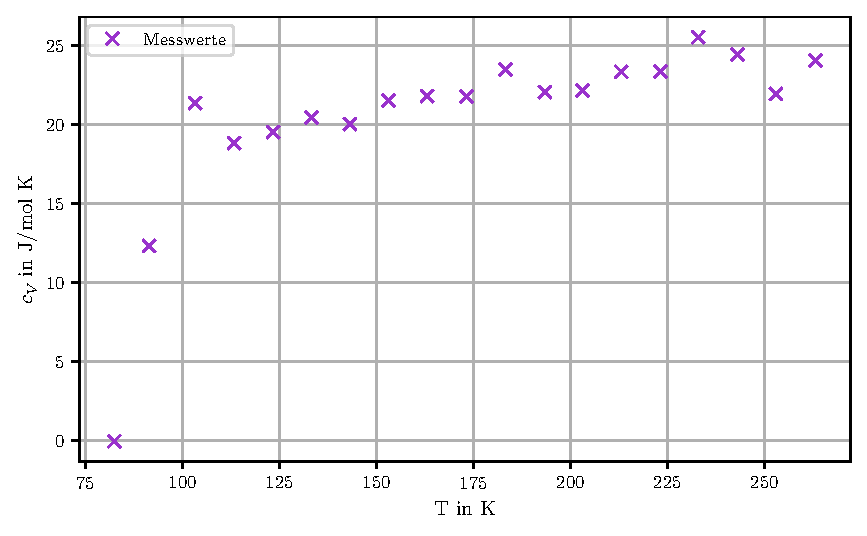
\includegraphics[width=0.7\textwidth]{build/Cv.pdf}
	\caption{The molar heat capacity $C_v$ as a function of temperature}
	\label{fig:heat_capacity_plot}
\end{figure}

\subsection{Experimental Debye Temperature}
\label{sec:experimental_debye_temperature}
